\chapter{Coordination in the Swarm}

\paragraph*{}
This section talks about the lower level of robot coordination after the target object is found, and all robots surround it securely. Firstly, our robot can be controlled based on the dynamic model of an omnidirectional wheeled mobile robot. This allows our robots to obtain holonomic motion, the ability to move in the given x-y direction instantaneously without changing its pose. Hence, our team came up with a coordination method by taking advantage of holonomic constraints to plan the movements for each robot to move the target object.

<<<<<<< HEAD
Our model works on the assumption that all robots will not change their relative pose relative to the object, such that they move collectively like one solid object where the center is the object's centroid. For simplicity in the calculation, we assume that all robot is equally distributed around the object (Figure \ref{fig:coordination-diagram}).
=======
\ref{fig:coordination-diagram}.
>>>>>>> 29614b76292cbe74150dd72ecf077680826f0b43

\begin{figure} [H]
    \centering
    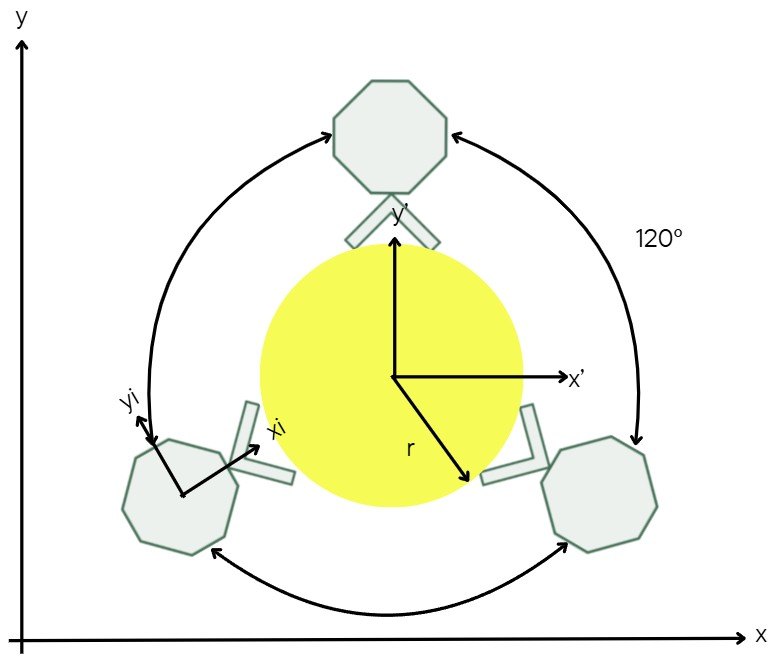
\includegraphics[width=0.3\linewidth]{assets/images/coordination/robots_with_object.jpg}
    \caption{Robots and the object in global frame}
    \label{fig:coordination-diagram}
\end{figure}

Then, our main objective is to make the object traverse a given trajectory. For that, our robots translate the trajectory into their own using their positions and geometric constraints. Given that \( r \) is the distance from the robot's centroid to the object's centroid, and \( \theta_i \) is the orientation of the \( i \)-th robot with respect to the object's frame, each robot adjusts its movement accordingly to maintain coordination in the system.

\[
J_i =
\begin{bmatrix}
1 & 0 & r \sin(\theta + \theta_i) \\
0 & 1 & r \cos(\theta + \theta_i) \\
0 & 0 & 1
\end{bmatrix}
\]

Each robot's position is determined using a Jacobian transformation that accounts for its relative displacement from the central reference point. This transformation considers the robot's angular offset and the radius of formation, ensuring that each robot maintains its relative position within the structure while responding to the overall system's movement. The Jacobian matrices allow the calculation of linear and angular velocities for each robot, ensuring accurate position updates over time.

These estimated velocities are included into the motion update equations to iteratively modify the orientation and position of every robot. The simulation represents the ongoing change of the motion of the system through discrete time increments. This makes it possible to observe the coordinated movement in which the robots dynamically modify their paths while maintaining the integrity of the formation.

These are results in MATLAB simulation:

\begin{figure}[!htb]
    \minipage{0.5\textwidth}
        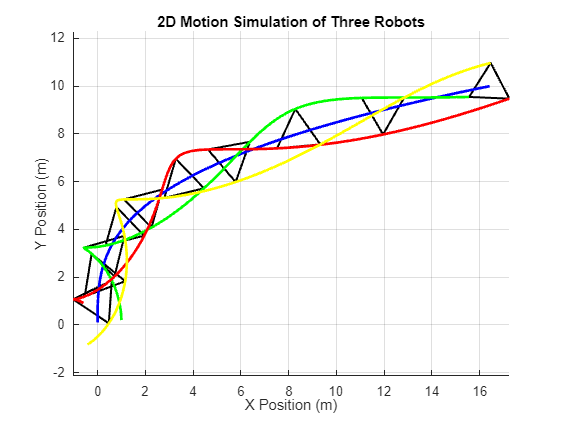
\includegraphics[width=\linewidth]{assets/images/coordination/parabolic.png}
        \caption{Parabolic function trajectory}
    \endminipage\hfill
    \minipage{0.5\textwidth}%
        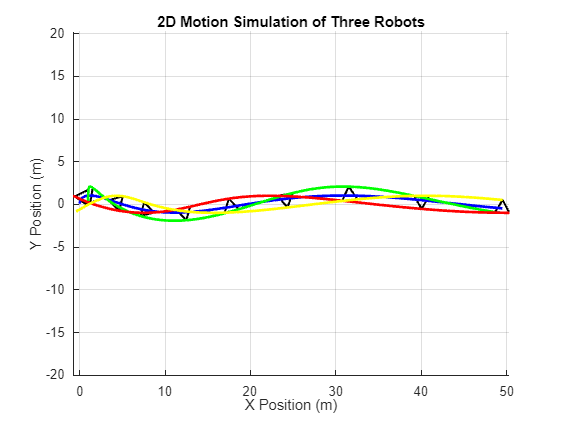
\includegraphics[width=\linewidth]{assets/images/coordination/sine.png}
        \caption{Sine function trajectory}
    \endminipage
\end{figure}
